\chapter{Background} \label{sec:background}

This chapter provides some background theory on the problem. It describes the electrical grid, the function of a transformer, 
the effect of modern appliances on the transformer and modelling of this effect. It draws heavily from the work of \cite{vanDijk2022}.

\section{Electrical grid}
\label{sec:grid}
Power generated at dams, nuclear power- and coal plants is transmitted to the consumer through the electrical grid. The grid is a network of power lines, transformers and other equipment. 
The grid is divided into three parts: generation, transmission and distribution. All these components are displayed in
figure \ref{fig:grid}.
\begin{figure}[H]
    \centering
    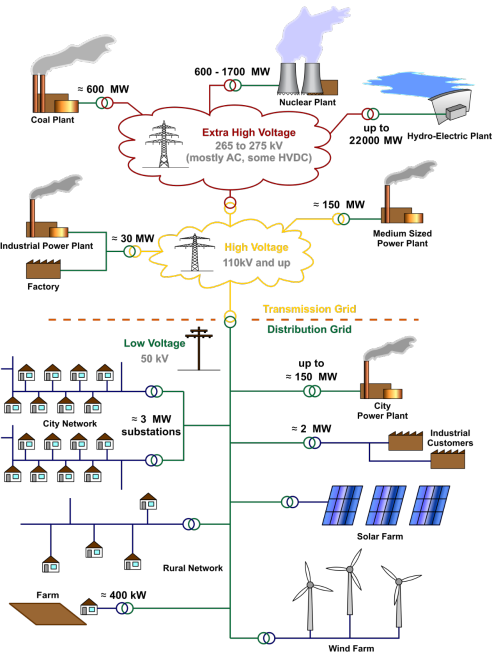
\includegraphics[width=0.5\textwidth]{img/distribution grid.png}
    \caption{Electricity grid \cite{mBizon2010}.}
    \label{fig:grid}
\end{figure} 
In the Netherlands specifically, the grid is divided into three voltage levels: extra high voltage, high voltage and low voltage.
The transmission grid ensures this high voltage ends up at factories, large power transformers and additional power is extracted from industrial and medium sized power plants.
Moreover, it is managed by a Transmission System Operator (TSO). 

Similarly, the distribution grid connects the transmission grid, cities, the rural network, solar-, wind farms to each other. It, in turn is managed by a Distribution System Operator (DSO)
In this paper the focus is on the transformers in the distribution grid. Figure \ref{fig:transformer} shows an example of such an transformer. This is because the distribution grid is the last part of the grid before the consumer. 
Consequently, the effects of modern appliances are most prominent in these types of transformers.
\begin{figure}[H]
    \centering
    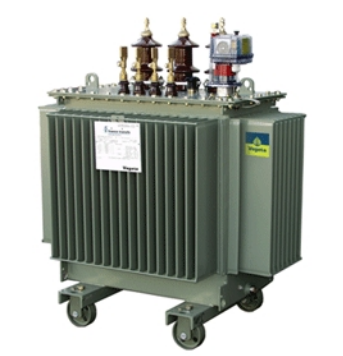
\includegraphics[width=0.5\textwidth]{img/transformer.png}
    \caption{Transformer \cite{dGebouwd2021}}
    \label{fig:transformer}
\end{figure}
The main goal of any transformer is to allow for the transmission of electrical energy over long distances. 
It achieves this by either increasing or decreasing voltage. In the former case, it is called a step-up transformer, in the latter case a step-down transformer.
A step-up tranformer allows for long distance transmission of electrical energy because the power loss is proportional to the current squared, which is decreased for increased voltage.
On the other hand, a step-down transformer is used to decrease the voltage to a level that is safe for the end-consumer.

\section{Workings of transformer}
A transformer is a device that transfers electrical energy from one circuit to another through inductively coupled conductors. 
It has three main components: a primary coil, a secondary coil and a core (see Figure \ref{fig:transformercore}). 
The primary coil is connected to the source of the electrical energy, the secondary coil is connected to a load and the core is made from a ferromagnetic material.
In the case of a distribution transformer, the primary coil is connected to the transmission grid and the secondary coil is connected to the distribution grid.
\begin{figure}[H]
    \centering
    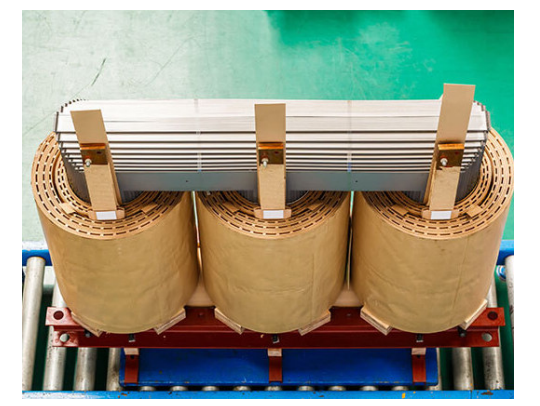
\includegraphics[width=0.5\textwidth]{img/transformercore.png}
    \caption{Main components of a transformer: primary (outer) coil, secondary (inner) coil and core. The coils are wound around the core
    and are wrapped in insulation themselves \cite{sSatsangi}.}
    \label{fig:transformercore}
\end{figure}

The insulation around the coils is necessary to prevent short-circuiting. Hence the lifetime of a transformer is limited by the lifetime of the insulation.
The latter in turn is determined by the amount of heat generated in the transformer. This heat is dissiapted through the core and the coils, where the core is the main contributor.
Therefore, this paper focusses on modelling the magnetic field generated in the core. 
The core losses and subsequent temperature profile may then be calculated from this magnetic field using the Steinmetz equation \cite{steinmetzEq},
\cite{vanDijk2022}.

\section{Higher Harmonics}
As stated in Section \ref{sec:grid}, the effect of modern appliances like computers, LEDs, solar panels and electric cars is most prominent in the distribution grid.
LEDs, for instance, are non-linear loads, which means they draw a current that is composed of a fundamental frequency and higher harmonics.
These higher harmonics are multiples of the fundamental frequency. The effect of these higher harmonics is that the current is no longer sinusoidal, but has a distorted shape.
This distortion is shown in Figure \ref{fig:higherharmonics}.
\begin{figure}[H]
    \centering
    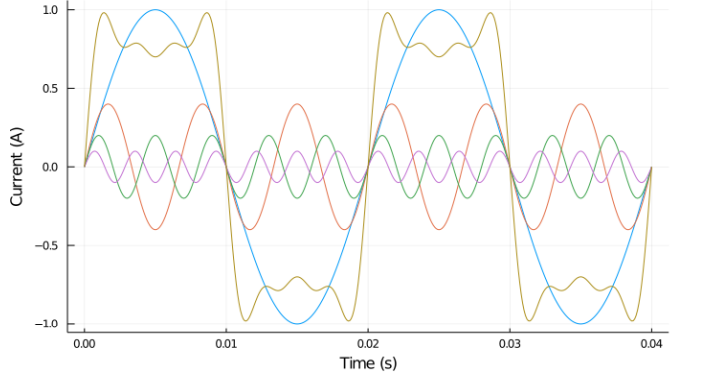
\includegraphics[width=0.5\textwidth]{img/higher_harmonics.png}
    \caption{Distorted current waveform \cite{vanDijk2022}.}
    \label{fig:higherharmonics}
\end{figure}
The magnetic field in the core depends on the frequency. A concrete example of this is the skin effect, which is the tendency of an alternating electric current to become distributed within a conductor 
such that the current density is largest near the surface of the conductor, and decreases with greater depths in the conductor.
The depth at which the current density is 37\% of the current density at the surface is called the skin depth. It is given by \citehere
\begin{equation}
    \delta = \sqrt{\frac{2}{\omega \mu \sigma}},
\end{equation}
which becomes smaller for larger frequencies. Hence, the skin effect is more prominent for higher harmonics. Therefore, more magnetic flux is generated in the outer layers of the core, leading to a higher loss, as well as a lower permeability. A numerical result is given in \cref{tab:skin_effect}

\begin{table}
    \centering
    \begin{tabular}{l|l}
        Frequency & $\delta$ \\
        \hline
        50 Hz   & 7.1 \\
        100 Hz  & 5.0 \\
        150 Hz  & 3.6 \\
        500 Hz  & 2.2 \\
        1000 Hz & 1.6 \\
    \end{tabular}
    \caption{Numerical values for the skin effect at different frequencies, with $\mu = \mu_r\mu_0 \approx 1000 \cdot 4e^{-7} \pi \approx 1.26e^{-3}, \sigma = 0.1$.}
    \label{tab:skin_effect}
\end{table}


\section{Permeability of the core}
Another complication in modelling the magnetic field in the core is that the permeability of the core is not constant for sufficiently large magnetic fields.
This is called the saturation of the core. The permeability of the core is given by
\begin{equation}
    \mu = \mu_0 \mu_r,
\end{equation}
where $\mu_0$ is the permeability of free space and $\mu_r$ is the relative permeability of the core. The permeability is a function of the magnetic field strength $H$.
The magnetic field strength is given by
\begin{equation}
    H = \frac{B}{\mu},
\end{equation}
where $B$ is the magnetic flux density. 

From this it follows that we can derive $\mu$ given we know the relation between $B$ and $H$. 
This relation is called the B-H curve, an example of which is visible in Figure \ref{fig:bhcurve}.
\begin{figure}[H]
    \centering
    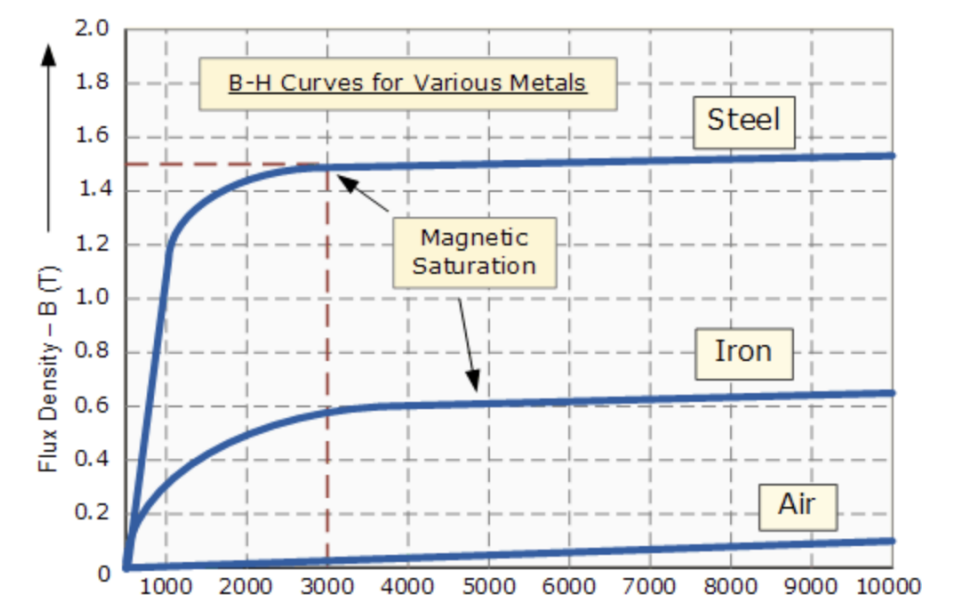
\includegraphics[width=0.5\textwidth]{img/BH_curve.png}
    \caption{B-H curve for various metals. $\mu$ is the slope of this curve. Once $\mu$ becomes nearly zero, the material is said 
    to be the saturated \cite{bhcurve}.}
    \label{fig:bhcurve}
\end{figure}

